\section{Knowledge of the Future}

In the last book of his Consolations of Philosophy, \textbf{Boethius} discusses how God can know the future if man is free. Recall how he explained the four levels of knowledge\footnote{\url{https://www.gornahoor.net/?p=5098}}: sense impressions, imagination, rational knowledge, and intuition. It is worth the effort to understand his explanation if for no other reason that intuition is critical for the man of Tradition. It cannot be learned from reading about it, but each man must develop it himself. The seeming contradiction involved in the dilemma can be treated as a type of koan that needs to be meditated on, while being elusive to rational thought. Curious readers may notice that this question arose again a millennium later in the dispute about Molinism\footnote{\url{https://en.wikipedia.org/wiki/Molinism}}. That dispute took the form of rational knowledge which Boethius firmly rejects as an adequate explanation. This demonstrates how metaphysical understanding gradually eroded over those 1000 years.

\begin{wrapfigure}{rt}{0.35\textwidth}
 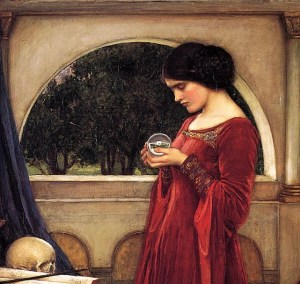
\includegraphics[scale=.5]{a20121210KnowledgeoftheFuture-img001.jpg} 
\end{wrapfigure}

This knowledge of the future baffles the rational mind, since it claims that the future can be known only if it be predetermined. However, this is a misunderstanding of what it means “to know”, since it places knowability in the object of knowledge rather than in the knower himself. Hence we are compelled to not consider the thing known, but rather we need to grasp how the knower knows. Following Augustine and the Neo-Platonists (and anticipating Rene Guenon, to be sure), Boethius first distinguishes between eternity and everlastingness. The latter is perpetual existence in time, whereas the former is outside time altogether. Boethius explains:

\begin{quotex}
The world is still not such that it may properly be considered eternal … Its life may be infinitely long, but it does not embrace and comprehend its whole extent simultaneously. It still lacks the future, while already having lost the past. So that that which embraces and possesses simultaneously the whole fullness of everlasting life, which lacks nothing of the future and has lost nothing of the past, that is what my properly be said to be eternal. … It is one thing to progress through everlasting life, and another thing to have embraced the whole of everlasting life in one simultaneous present. This is clearly a property of the mind of God. 

\end{quotex}
Boethius follows Plato's claim that “God is eternal, the world perpetual.” For the world, the past is always receding (“lost”) while the future is not yet (“lacking”). Thus God cannot be considered as existing “before” the world. Hence, it is not really a question of foreknowledge of the future, but instead the “knowledge of a never ending presence.” This is the literal meaning of Providence, “looking forth”, which he contrasts to prevision or “seeing ahead”.

Next, Boethius addresses the counterargument that to know future events implies that the future is determined and free will is not possible. Obviously, this is mechanical thinking arising from the rational mind as opposed to the organic thinking that sees time as a whole. If I watch you walking down the street, then I know it through sense perception; nevertheless, this type of knowing, which is also a form of direct intuition, does not make your perambulation unfree or necessary.

By analogy, and that is all we may have for now, the same can be said about God's seeing through intellectual intuition. Boethius writes:

\begin{quotex}
Divine foreknowledge does not change the nature and property of things; it simply sees things present to it exactly as they will happen at some time as future events. … the divine gaze looks down on all things without disturbing their nature; to Him, they are present things, but under the conditions of time they are future things. And so when God knows that something is going to occur and knows that no necessity to be is imposed on it, it is not opinion, but rather knowledge founded upon truth. 

\end{quotex}
In the example of watching someone walk on the street, we were clearly appealing to spatial perception rather than temporal. It is easy to grasp that our experience of objects in space is grasping the whole, as something all-at-once, at least within the limits of our horizon. But events in time don't typically have that same effect, as events come at us sequentially, not all at once. Each moment in time seems independent of what follows; this is what perplexed Hume so that he could not understand the nature of causality. Yet as we recently pointed out\footnote{\url{https://www.gornahoor.net/?p=5381}}, artistic inspiration often takes this form. This is why Solovyov used artistic experience as the model for the type of intuition being described. In particular music and poetry lend themselves to this, this they unfold in time while being grasped as a whole. Hence, we can grasp a symphony as a whole even though our experience is one note after another. Yet, the musicians play the instruments by their own free will.

It may be helpful to draw on what \textbf{Rene Guenon} writes about time in The Reign of Quantity. He points out that time is more subtle than space, and that accounts for its elusiveness. It can only be measured by spatial criteria and the most intimate part of us — our mental life — develops in time yet has no spatial character. This means that time is even more qualitative than space and our tendency to experience time just in its quantitative aspect can only result in misunderstanding. Guenon uses the example of the four seasons, the temporal equivalent of the four spatial directions. Once we see things in terms of cycles — organically — we can “predict” the future. Of course, the world unfolds in cycles within cycles, etc.

Next, we can point out the nature of manifestation. Recall that a fundamental principle is the identity of knowing and being. We know that there are possibilities of manifestation. When God knows a possibility of manifestation, as he must since it is an idea in His own mind, then it necessarily manifests—essence and existence are one. And this is so, even if from the perspective of time, it is the result of free acts.

Finally, how can man experience things \emph{sub specie aeternitatis}? Obviously, not man qua man, but only from states that are higher than the human state. To reach that highest state is what Guenon calls deliverance as opposed to salvation. Readers who continue to do their exercises and meditations may find that they can reach a state of detachment in which consciousness is observing the actions of the body. Within the incessant states of conscious activity, that is, the everlasting or perpetual, what is the one constant? That is the eternal.



\flrightit{Posted on 2012-12-10 by Cologero }

\begin{center}* * *\end{center}

\begin{footnotesize}\begin{sffamily}



\texttt{Saladin on 2013-10-18 at 13:25 said: }

Very interesting! I have just discovered The Consolation of Philosophy, and it is a real gem!


\end{sffamily}\end{footnotesize}
